%
% richtungsfeld.tex
%
% (c) 2020 Prof Dr Andreas Müller, Hochschule Rapperswil
%
\begin{frame}[fragile]
\frametitle{Differentialgleichung und Richtungsfeld}
\begin{columns}[t]
\begin{column}{0.48\hsize}
\begin{block}{Differentialgleichung}
\vspace{-18pt}
\begin{align*}
y' &= y - x = f(x,y)
\\
y(0) &= y_0
\end{align*}
\end{block}
\vspace{-15pt}
\uncover<2->{%
\begin{block}{Richtungsfeld}
In jedem Punkt $(x,y)$ eine Gerade mit  Steigung $f(x,y)$
\end{block}}
\uncover<3->{%
\begin{block}{Lösung}
Der Graph von $y(x)$ hat in jedem Punkt Richtungsfeld als 
Tangente
\end{block}}
\end{column}
\begin{column}{0.48\hsize}
\begin{center}
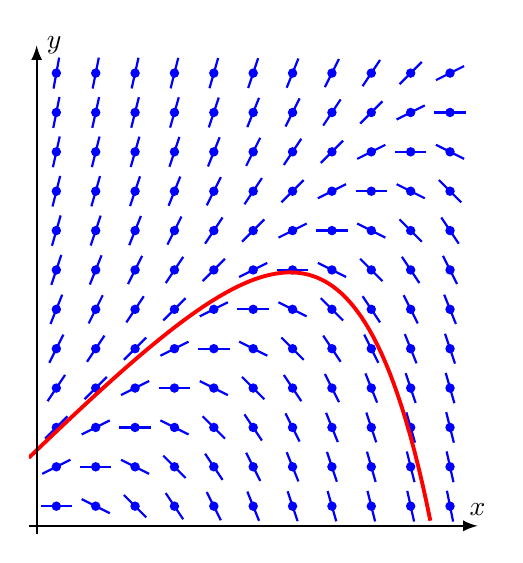
\begin{tikzpicture}[>=latex,thick]

\def\steigung#1#2{
	\pgfmathparse{\y-\x}
	\xdef\yprime{\pgfmathresult}
	\pgfmathparse{atan(\yprime)}
	\xdef\a{\pgfmathresult}
	\fill[color=blue] (#1,#2) circle[radius=0.06];
	\draw[color=blue]
		({#1-0.2*cos(\a)},{#2-0.2*sin(\a)})--
		({#1+0.2*cos(\a)},{#2+0.2*sin(\a)}) ;
}

\uncover<2->{
\foreach \x in {0.25,0.75,...,5.5}{
	\foreach \y in {0.25,0.75,...,6}{
		\steigung{\x}{\y}
	}
}
}

\uncover<3->{
\begin{scope}
\clip (-0.1,-0.1) rectangle (5.4,6);
\draw[color=red,line width=1.4pt] plot[domain=-0.1:5,samples=100]
	({\x},{1+\x+(0.96-1)*exp(\x)});
\end{scope}
}

\draw[->] (-0.1,0)--(5.6,0) coordinate[label={$x$}];
\draw[->] (0,-0.1)--(0,6.1) coordinate[label={right:$y$}];
\end{tikzpicture}
\end{center}
\end{column}
\end{columns}
\end{frame}
